\subsubsection{CAD input files}
\begin{frame}{CAD input files}

\begin{enumerate}
\item Optimization domain
\begin{itemize}
\item Fixture faces 
\item Forces
\end{itemize}
\end{enumerate}

%Red faces (RGB=[255,0,0]): Fixture
%\item Green faces (RGB=[0,255,0]): Non-changing region  
%\item Colored (RGB=[0-255,0-255,0-255]): 3D loading vector 
%Linear force scaling: $F=f*({\bf x}-127)$\\
%One Byte: 0-126 negative, 127 zero, 128-255 positive direction
\begin{figure}
\centering
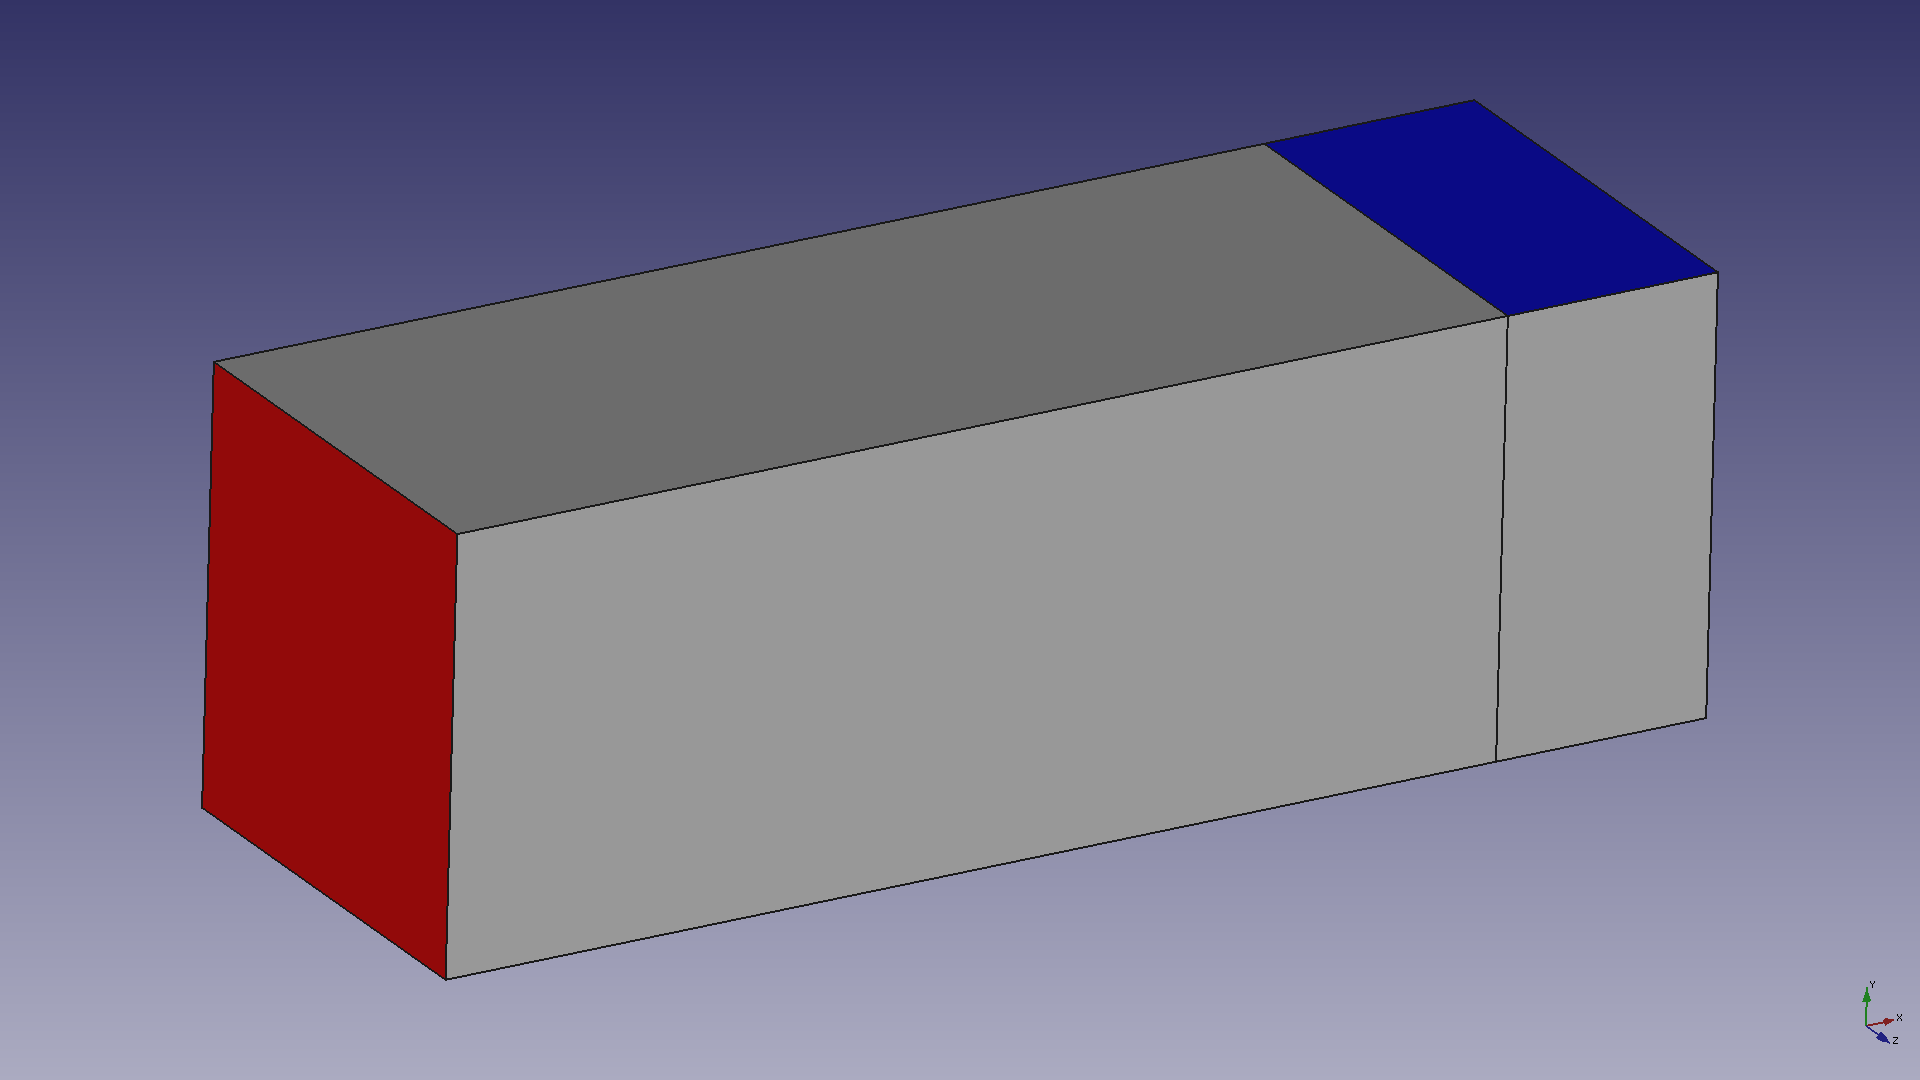
\includegraphics[width=.5\textwidth]{Pictures/CantileverColored.png}
\end{figure}
\end{frame}

\subsubsection{Voxelization}
\begin{frame}{Voxelized geometry}
\begin{itemize}
\item OpenCascade STEP/IGES CAF reader 
\item Voxelize faces/geometry seperately: Boolean (0/1) grid for 
\begin{enumerate}
\item Active voxels (geometry)
\item Fixture voxels
\item Non-changing voxels
\item Load voxels
\end{enumerate}
\end{itemize}
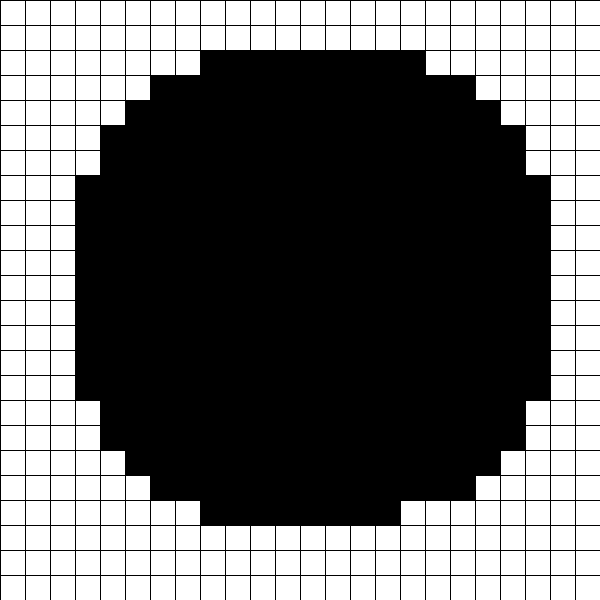
\includegraphics[width=.25\textwidth]{Pictures/Active.pdf}
\hspace{1cm}
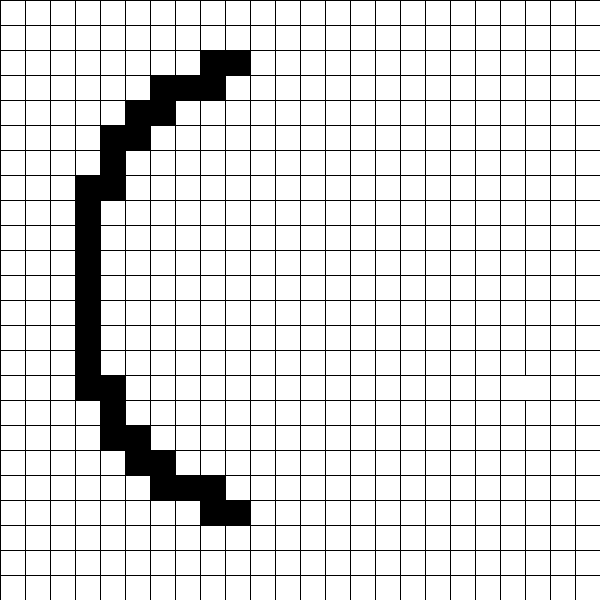
\includegraphics[width=.25\textwidth]{Pictures/NonChanging.pdf}
\hspace{1cm}

\includegraphics[width=.25\textwidth]{Pictures/Load.pdf}
\end{frame}

\subsubsection{Black-Box Toplogy Optimizer}
\begin{frame}{Topology Optimization Process}
\begin{center}
Provide geometry as voxel grid
$$\downarrow$$
Calculate stress on each voxel
$$\downarrow$$
Remove voxel from active geometry if stress is below threshold
\end{center}
\end{frame}

\begin{frame}{Topology Optimization Example}

\only<1>{
\begin{figure}
\centering
%\vspace{-0.5cm}
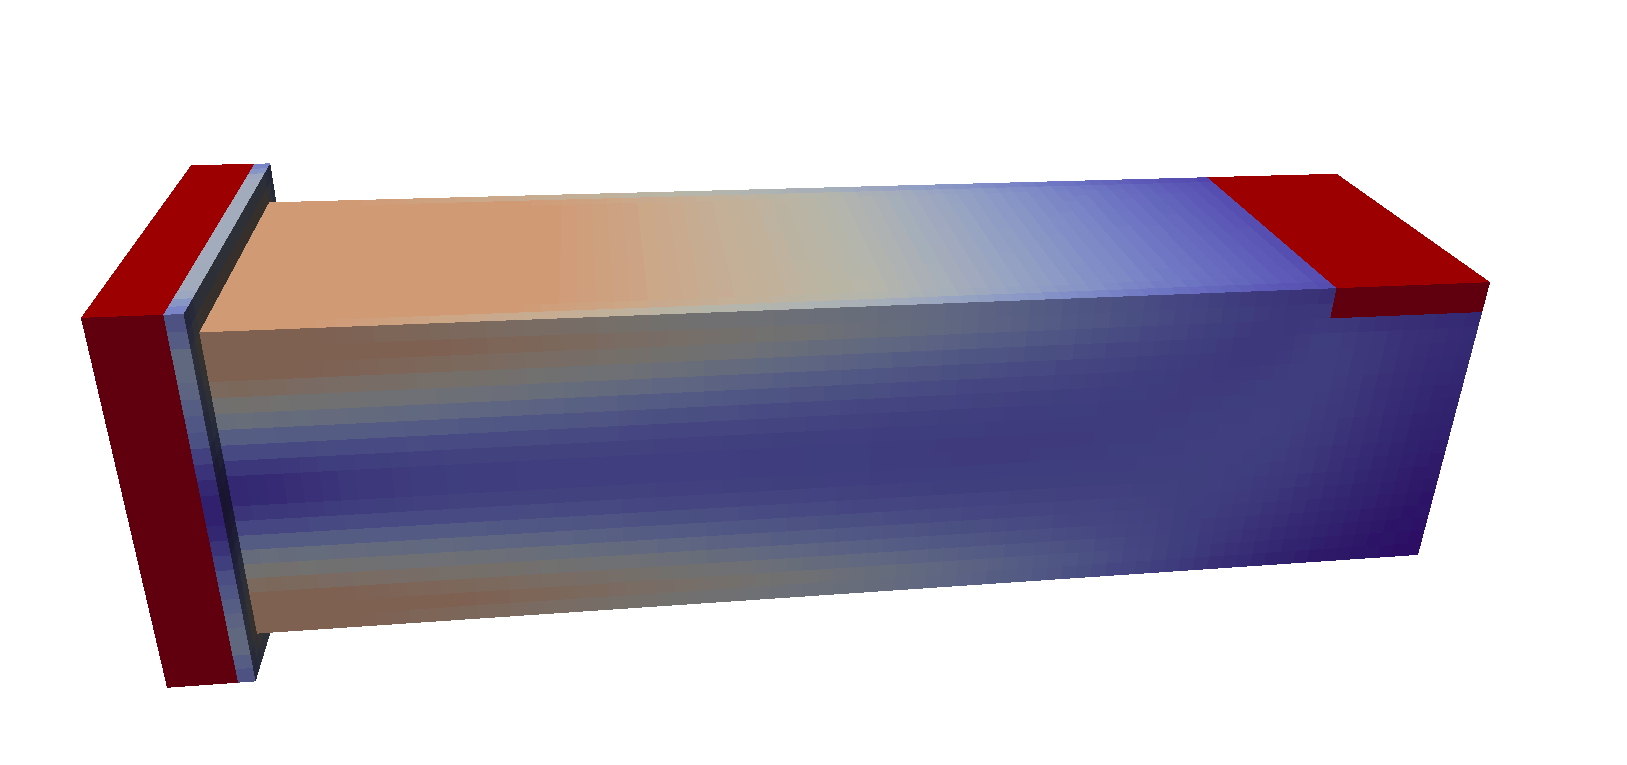
\includegraphics[width=1\textwidth]{Pictures/SecondHalf/Topology/Cantilever_Topy_0.png}
\end{figure}}
\only<2>{
\begin{figure}
\centering
%\vspace{-0.5cm}
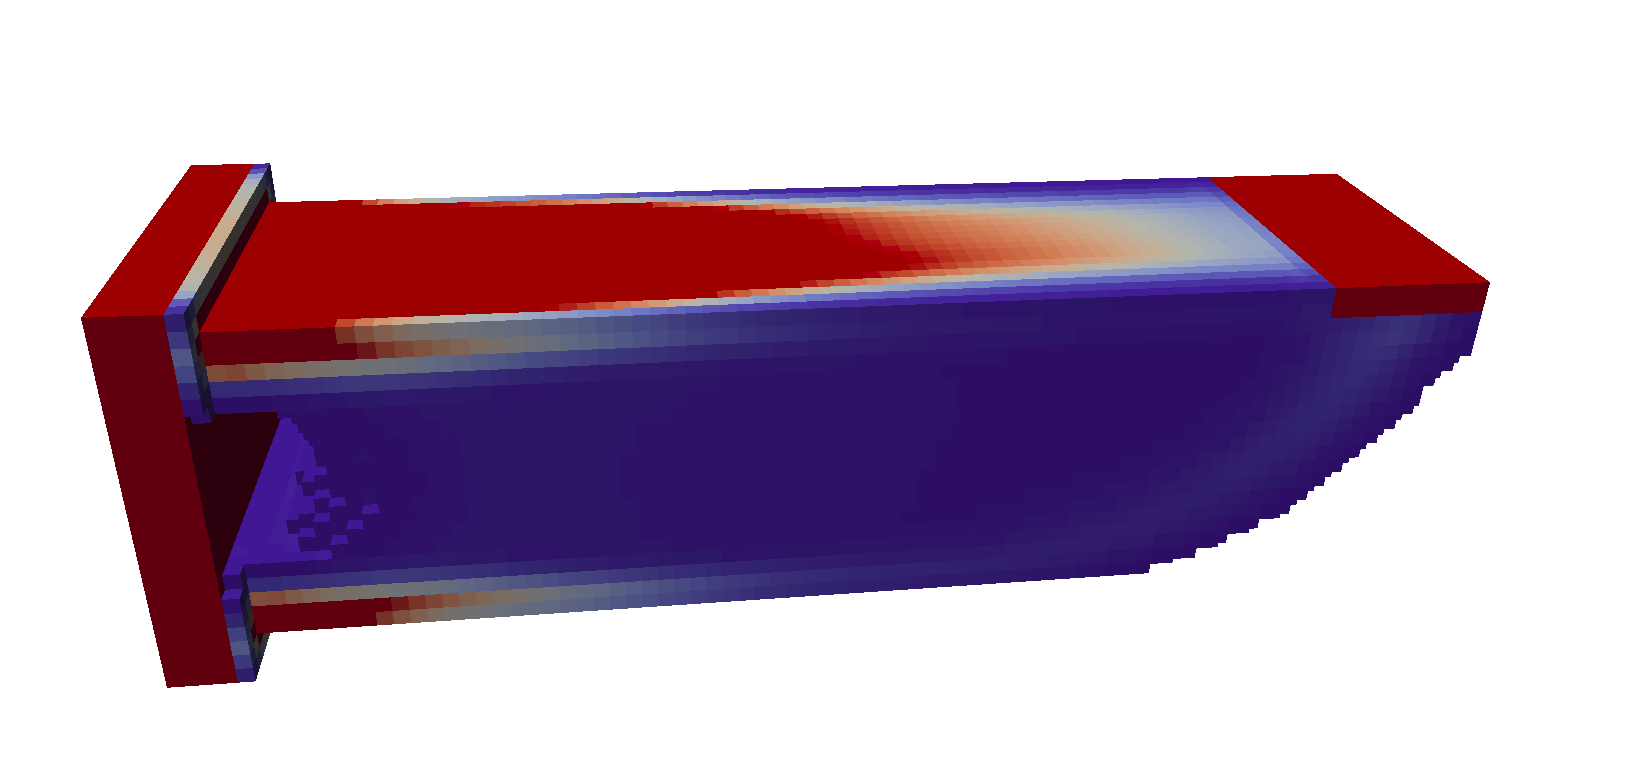
\includegraphics[width=1\textwidth]{Pictures/SecondHalf/Topology/Cantilever_Topy_1.png}
\end{figure}}
\only<3>{
\begin{figure}
\centering
%\vspace{-0.5cm}
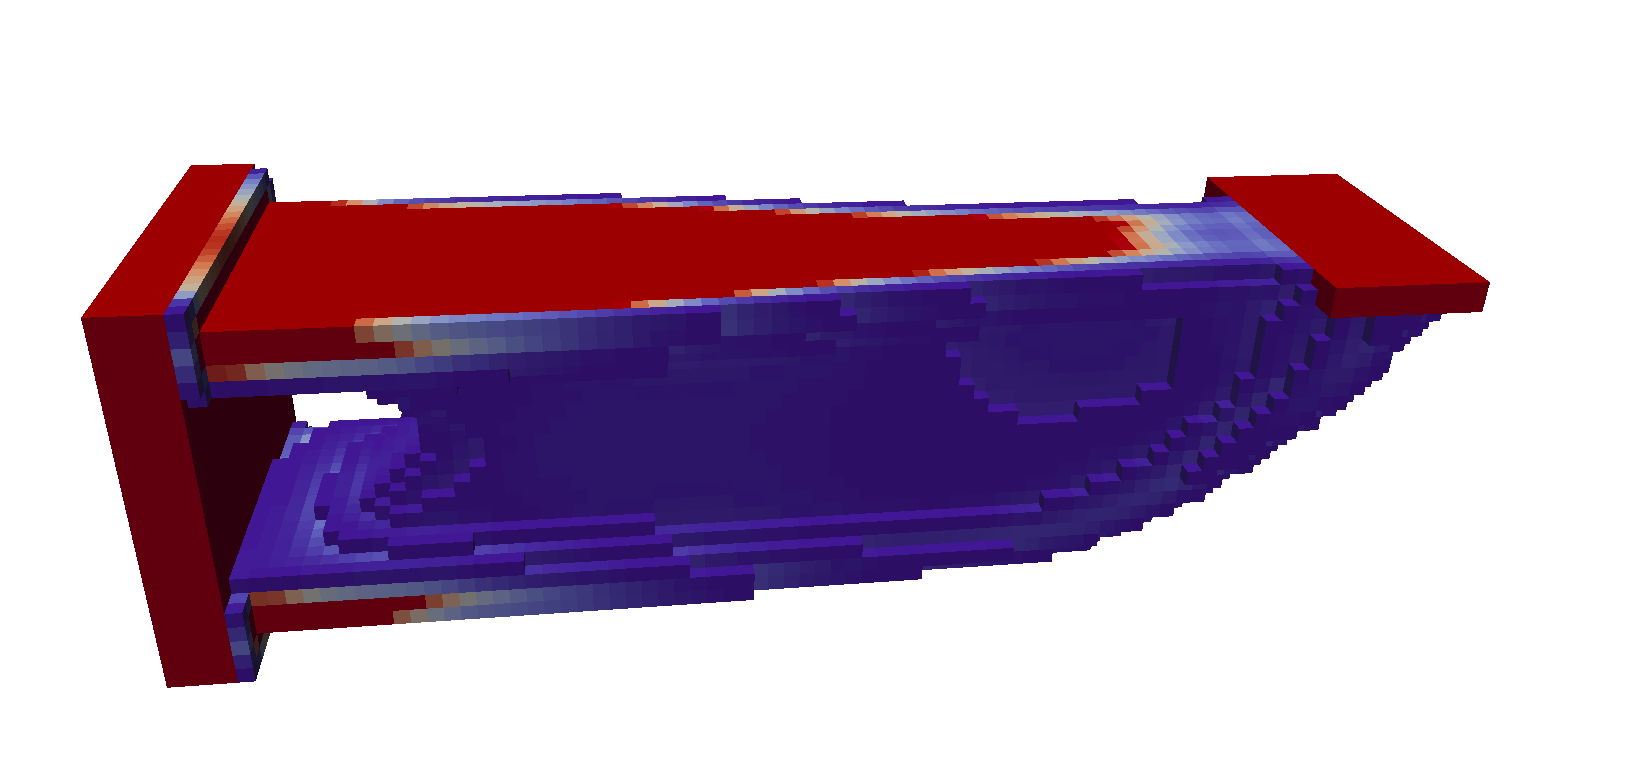
\includegraphics[width=1\textwidth]
{Pictures/SecondHalf/Topology/Cantilever_Topy_2.png}
\end{figure}}
\only<4>{
\begin{figure}
\centering
%\vspace{-0.5cm}
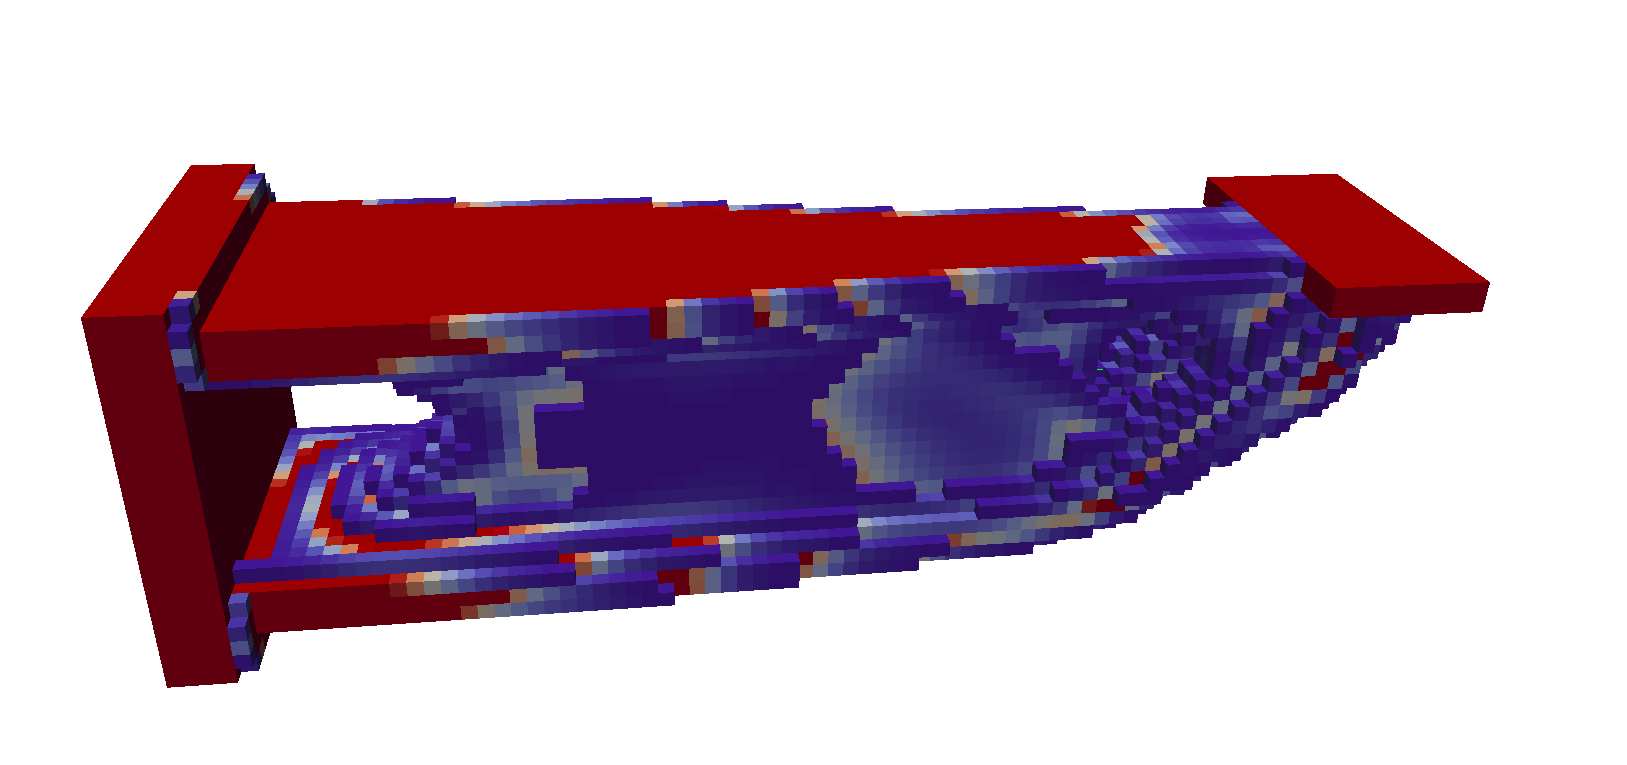
\includegraphics[width=1\textwidth]{Pictures/SecondHalf/Topology/Cantilever_Topy_3.png}
\end{figure}}
\only<5>{
\begin{figure}
\centering
%\vspace{-0.5cm}
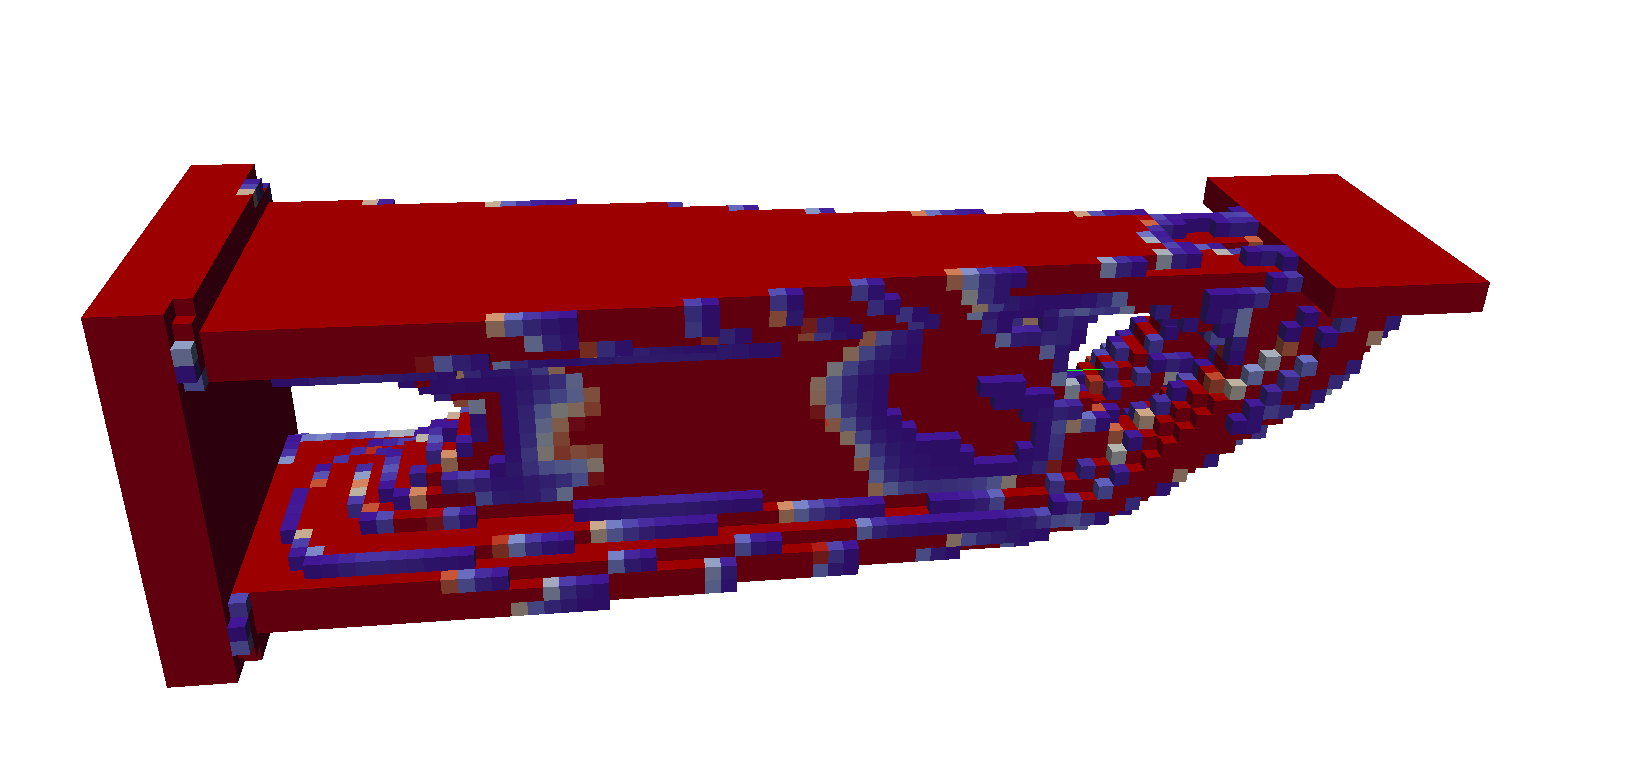
\includegraphics[width=1\textwidth]{Pictures/SecondHalf/Topology/Cantilever_Topy_4.png}
\end{figure}}
\only<6>{
\begin{figure}
\centering
%\vspace{-0.5cm}
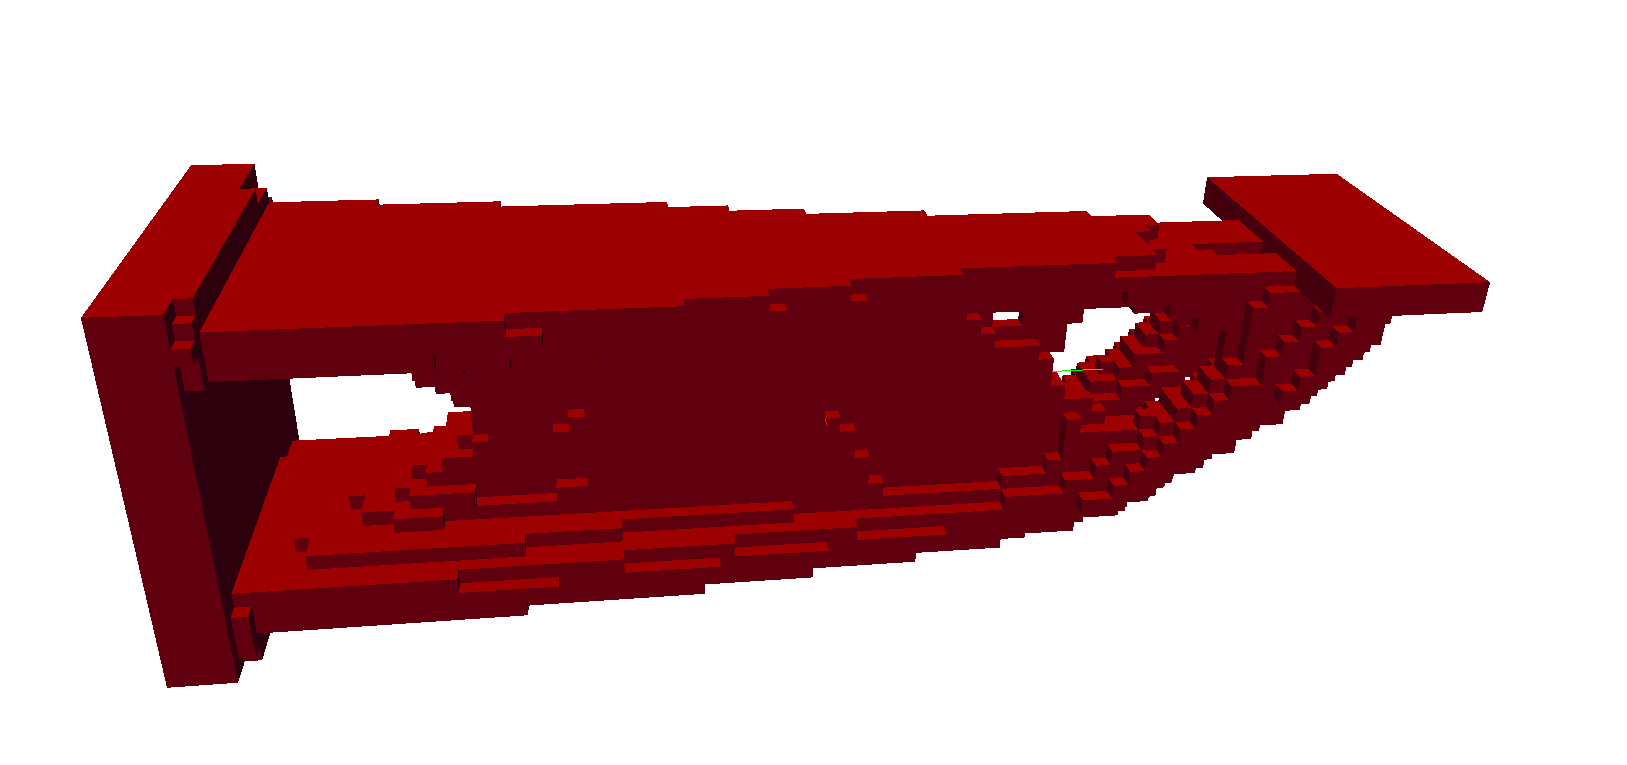
\includegraphics[width=1\textwidth]{Pictures/SecondHalf/Topology/Cantilever_Topy_5.png}
\end{figure}}
\end{frame}
